\documentclass[10pt]{beamer}

% mac版,texShop 中Typeset选择 XeLaTex 

%%%%%%%%%%%%%%%%%%%%%%%%%%%%%%%%%%%%%
\usepackage[slantfont,boldfont]{xeCJK}
%\input{xecjkfonts},CJKtextspaces
\setCJKmainfont{STKaiti}   % STFangsong 设置缺省中文字体
\setCJKmonofont{SimSun}   % 设置等宽字体
\setmainfont{Times} % 英文衬线字体
\setmonofont{Times} % 英文等宽字体
\setsansfont{Times} % 英文无衬线字体
%%%%%%%%%%%%%%%%%%%%%%%%%%%%%%%%%%%%%%

\mode<presentation> {
  %\usetheme{Madrid}
  %\usetheme{Singapore}
  \usetheme{Warsaw}
  \setbeamercovered{transparent}
 % \usefonttheme[onlymath]{serif}  
 \usefonttheme{professionalfonts}%{structurebold}
 % \usefonttheme[onlymath]{structurebold}
  \usecolortheme{rose}
}

\usepackage[english]{babel}
%\usepackage[latin1]{inputenc}

%\usepackage{times}
%\usepackage[T1]{fontenc}


%\usepackage{epsfig}
\usepackage{graphics}
\usepackage{color}
\usepackage{amsmath,amssymb,mathrsfs}
\usepackage{amsfonts,stmaryrd}
%\usepackage{thmmarks}
%\usepackage{}



\newcommand\frakfamily{\usefont{U}{yfrak}{m}{n}}
\DeclareTextFontCommand{\textfrak}{\frakfamily}
\def\diag{\mathrm{diag}}


\title[数值计算方法]{数值计算方法}
\subtitle{-最小二乘问题}


\subject{Talks}

% If you have a file called "university-logo-filename.xxx", where xxx
% is a graphic format that can be processed by latex or pdflatex,
% resp., then you can add a logo as follows:

% \pgfdeclareimage[height=0.5cm]{university-logo}{university-logo-filename}
% \logo{\pgfuseimage{university-logo}}

%\pgfdeclareimage[height=0.5cm]{university-logo}{ncsu_logo}
%\logo{\pgfuseimage{university-logo}}

% Delete this, if you do not want the table of contents to pop up at
% the beginning of each subsection:
%\AtBeginSubsection[] {
%  \begin{frame}<beamer>
%    \frametitle{Outline}
%    \tableofcontents[currentsection,currentsubsection]
%  \end{frame}
%}

% If you wish to uncover everything in a step-wise fashion, uncomment
% the following command:

% \beamerdefaultoverlayspecification{<+->}


\setbeamertemplate{theorems}[numbered]
\setbeamertemplate{caption}[numbered]


\newtheorem{proposition}[theorem]{Proposition}

%%%%%%%%%%%%%%%%%%%%%%%%%%%
% REMARK-STYLE-ENVIRONMENTS %
%%%%%%%%%%%%%%%%%%%%%%%%%%%
\newcounter{remark}
% \numberwithin{theorem}{section}
\def\openrem#1#2{\refstepcounter{remark}\bigskip

{\noindent\bf#1~\theremark\if#2!{. }\else{ (#2).}\fi}
\it}
\def\thmskip{}
\newenvironment{remark}[1][!]{\openrem{Remark}{#1}}{\thmskip}

%%%%%%%%%%%%%%%%%%%%%%%%%%%%
%% AlGORITHM-STYLE-ENVIRONMENTS %
%%%%%%%%%%%%%%%%%%%%%%%%%%%%
\newcounter{algorithm}
% \numberwithin{theorem}{section}
\def\openalg#1#2{\refstepcounter{algorithm}\bigskip

{\noindent\bf#1~\thealgorithm\if#2!{. }\else{ (#2).}\fi}
\it}
\def\thmskip{}
\newenvironment{algorithm}[1][!]{\openrem{Algorithm}{#1}}{\thmskip}
%
%
%%%%%%%%%%%%%%%%%%%%%%%%%%%%
%% Result-STYLE-ENVIRONMENTS %
%%%%%%%%%%%%%%%%%%%%%%%%%%%%
%\newcounter{result}
%\def\openrem#1#2{\refstepcounter{result}\bigskip
%{\noindent \it \bfseries#1~\theremark\if#2!{. }\else{ (#2). }\fi}}
%\newenvironment{result}[1][!]{\openrem{Result}{#1}}{\qed}




%%%%%%%%%%%%%%%%%%%%%%%%%%%
%Redefine the Symbols%
%%%%%%%%%%%%%%%%%%%%%%%%%%%

\def\mathbi#1{\textbf{\em #1}}

% integrals
\def\dx{\,{\rm d}x}
\def\dxb{\,{\rm d}\boldsymbol{x}}
\def\dy{\,{\rm d}y}
\def\dt{\,{\rm d}t}
\def\ds{\,{\rm d}s}
\def\du{\,{\rm d}u}

\def\dr{\,{\rm d}r}
\def\dtheta{\,{\rm d}\theta}

\def\dd{{\rm d}}

\def\intOm{\int_{\Omega}}
\def\intbOm{\int_{\partial \Omega}}

% differences
\def\Dx{\Delta x}
\def\Dt{\Delta t}
\def\D{\Delta}


% operators
\def\Ls{\mathscr{L}}

% matirices
\def\Js{\mathscr{J}}


%fields%
\def\R{\mathbb{R}}
\def\N{\mathbb{N}}
\def\Z{\mathbb{Z}}

%Spaces%
\def\H{\mathbb{H}}
\def\L{\mathbb{L}}
\def\P{\mathbb{P}}


\def\U{\mathbb{U}}
\def\V{\mathbb{V}}
\def\W{\mathbb{W}}
\def\X{\mathbb{X}}
\def\Y{\mathbb{Y}}

\def\Cinfty{C^\infty}




%vectors%
\def\ab{\boldsymbol{a}}
\def\bb{\boldsymbol{b}}
\def\cb{\boldsymbol{c}}
\def\db{\boldsymbol{d}}
\def\eb{\boldsymbol{e}}
\def\fb{\boldsymbol{f}}
\def\gb{\boldsymbol{g}}
\def\hb{\boldsymbol{h}}
\def\nb{\boldsymbol{n}}
\def\rb{\boldsymbol{r}}
\def\sb{\boldsymbol{s}}


\def\ub{\boldsymbol{u}}
\def\vb{\boldsymbol{v}}
\def\wb{\boldsymbol{w}}
\def\xb{\boldsymbol{x}}
\def\yb{\boldsymbol{y}}
\def\zb{\boldsymbol{z}}

\def\Bb{\boldsymbol{B}}
\def\Cb{\boldsymbol{C}}
\def\Eb{\boldsymbol{E}}
\def\Fb{\boldsymbol{F}}
\def\Ib{\boldsymbol{I}}
\def\Kb{\boldsymbol{K}}
\def\Ob{\boldsymbol{O}}
\def\Qb{\boldsymbol{Q}}
\def\Rb{\boldsymbol{R}}
\def\Sb{\boldsymbol{S}}
\def\Ub{\boldsymbol{U}}
\def\Vb{\boldsymbol{V}}
\def\Wb{\boldsymbol{W}}
\def\Xb{\boldsymbol{X}}
\def\Yb{\boldsymbol{Y}}
\def\Zb{\boldsymbol{Z}}

%domains%
\def\Om{\Omega}
\def\bd{\partial}
\def\bOm{\bar{\Omega}}

%bold symbols%
\def\alphab{\boldsymbol{\alpha}}
\def\phib{\boldsymbol{\varphi}}

%energy%
\def\Jc{\mathcal{J}}
\def\Oc{\mathcal{O}}

%Greeks%
\def\vphi{\varphi}

%Special Functions%
\def\supp{\rm{supp}}
\def\sym{\rm{sym}}

\def\gradu{\nabla u}
\def\gradv{\nabla v}

%Mesh%
\def\Ts{\mathcal{T}}

\def\mach{\rm{mach}}


\begin{document}

\setbeamertemplate{itemize item}[triangle]

\begin{frame}
\titlepage
\end{frame}


\begin{frame}
  \frametitle{本节概要}
  \tableofcontents%[pausesections]
  % You might wish to add the option [pausesections]
%  \begin{itemize}
%  \item 显示Euler法及其误差分析
%  \item Taylor展开法
%  \item 
%  \end{itemize}
\end{frame}

\section{法方程的导出}

\begin{frame}
\frametitle{最小二乘问题概述}
最小二乘问题可以从两个不同的方面导出。

\vspace{0.2cm}

第一个方面是解线性方程组。我们之前讨论的解线性方程组的问题都一般都假设线性方程组的解存在且唯一,但是在科研和工程实践中,我们有时会遇到方程组个数大于未知数个数的情况,这种情况下方程往往是没有解的。我们解决这个问题的方法一般是在一定的意义下找到近似满足原方程的解,这一般指的就是最小二乘意义下的解。

\vspace{0.2cm}

第二个方面是数据的拟合。我们在插值法一章中严格的要求插值条件满足,也就是插值函数一定要通过所有的插值点。这样个要求一方面会导致插值函数次数升高,另一方面由于数据的测量总会包含误差,因此严格要求插值函数满足插值条件是不必要的。因此,我们往往使用最简单的函数寻找数据点中自变量与因变量之间关系的趋势。

\vspace{0.2cm}
\end{frame}

\begin{frame}
\frametitle{超定(不相容)方程}
考虑以下方程组
\begin{align}
\label{eq: least square eq 1}
x_1 + x_2 = 2, \nonumber \\
x_1 - x_2 = 1, \nonumber \\
x_1 + x_2 = 3.
\end{align}
我们发现这个方程组中第一个和第三个方程是不能够同时满足的。这样因为矛盾没有解的方程组一般称为超定的或者不相容的方程组。

\vspace{0.2cm}

不相容的方程组往往是由于方程个数$m$大于未知量的个数$n$造成的。虽然这样的方程不能够通过高斯消元等方法找到解,但是我们可以在某种意义下找到使得方程组左右两边近似相等的解。
\end{frame}


\begin{frame}
\frametitle{最小二乘解}
我们首先要给一个关于近似程度的度量。由于方程组的左右两边都是欧几里德空间$\R^n$上的向量,我们就用向量的欧几里得距离来度量两个向量的相似程度。使得方程两边的欧几里得距离最小的那个解就称为方程组的最小二乘解。

\begin{remark}
考虑两个向量$u = (u_1, u_2, \ldots, u_n)$,$v = (v_1, v_2, \ldots, v_n)$,则两个向量的欧几里得距离为
\begin{equation}
\|u - v\|_{2} = \big( (u_1-v_1)^2 + (u_2 - v_2)^2 + \ldots + (u_n - v_n)^2 \big)^{\frac{1}{2}}.
\end{equation}
根据这个定义,要使得两个向量的欧几里得距离最小,则需要使两个向量的二乘,即
\begin{equation}
(u_1-v_1)^2 + (u_2 - v_2)^2 + \ldots + (u_n - v_n)^2,
\end{equation}
最小。这就是为什么称满足上面所说条件的解为最小二乘解。
\end{remark}
\end{frame}


\begin{frame}
\frametitle{最小二乘的几何解释}
我们现在从几何的角度来看方程组\eqref{eq: least square eq 1}。我们将它写为$Ax = b$的形式
\begin{align}
&\left[ \begin{array}{cc}
     1    & 1 \\
     1    &   -1 \\
     1    &  1                          
            \end{array} \right] 
\left[ \begin{array}{c} 
      x_1 \\ x_2 \end{array} \right] 
=
\left[ \begin{array}{c}
     2 \\ 1 \\3  \end{array} \right].
\end{align}
这等价于
\begin{align}
\label{eq: least square 2}
x_1\left[ \begin{array}{c}
     1     \\
     1     \\
     1                           
            \end{array} \right] 
+
x_2\left[ \begin{array}{c}
     1     \\
     -1     \\
     1                           
            \end{array} \right] 
=
\left[ \begin{array}{c}
     2 \\ 1 \\3  \end{array} \right].
\end{align}
事实上,一个$m\times n$的矩阵$A$组成的线性方程组$Ax = b$可以看作是向量方程
\begin{equation}
\label{eq: least square 3}
x_1 v_1 + x_2 v_2 + \ldots + x_n v_n = b,
\end{equation}
其中$v_i$是$A$的第$i$列。也就是说,我们可以把解线性方程组考虑成为寻找用$A$的各列上的向量通过线性组合来将右端项$b$表示出来的办法,而$x_i$就是这些列向量线性组合的系数。
\end{frame}


\begin{frame}
\frametitle{最小二乘的几何解释}
考虑方程\eqref{eq: least square 2},这个方程无法满足的根本原因是向量$(2,1,3)^T$这个向量根本就不在$(1,1,1)^T$和$(1,-1,1)$这两个向量所张成的向量空间中。换句话说,一般来说要使得\eqref{eq: least square 3}的有解,则其右端项$b$必须处于$v_1, v_2, \ldots, v_n$张成的向量空间中。但是我们对$b$没有任何的控制,所以$b$可能在这个空间中,也可能不在这个空间中。下图表示了这两种情况
\begin{figure}
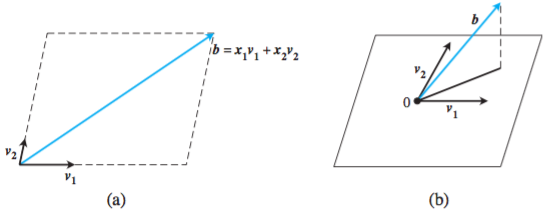
\includegraphics[width=11cm]{figs/4-1-1_Vector_Representation-1} 
%\caption{$f(x) = x^3 + x -1$的图像} 
\end{figure}
\end{frame}


\begin{frame}
\frametitle{最小二乘的几何解释}
方程组\eqref{eq: least square 2}就正如第二幅图一样,$b$不在$v_1,v_2$所张成的向量空间中。这时候由于方程组左边的向量一定处于$v_1,v_2$所张成的向量空间(平面)中,所以我们只能够在这个空间中找到(在欧几里得意义下)最接近于$b$的向量。

\vspace{0.2cm}

根据空间立体几何的基本定理,这个在$span\{ v_1, v_2\}$中最接近于$b$的向量正好是$b$向量作关于空间(平面)$span\{ v_1, v_2\}$的垂线与$span\{ v_1, v_2\}$空间(平面)的交点与原点连接所得到的向量,我们设这个向量是$\bar{b} =: A\bar{x}$。而根据空间立体几何的基本定理,$\bar{b}$还满足一个重要的关系,就是$b - \bar{b} \perp v, \forall v \in span\{ v_1, v_2\}$,即$\bar{b}$与空间(平面)垂直。

\vspace{0.2cm}

如果我们把以上空间立体几何的语言翻译成空间解析几何的语言,就得到
\begin{equation}
(b - \bar{b}) \cdot v,  \forall v \in span\{ v_1, v_2\}.
\end{equation}
由于$\bar{b} = A\bar{x}$,且由于$v \in span\{ v_1, v_2\}$,从而$\forall v, \exists x$使得$v = Ax$,我们有
\begin{equation}
\label{eq: least square 4}
 (b - A\bar{x}) \cdot Ax = (b - A\bar{x})^T  Ax = 0, \quad, \forall x \in \R^2.
\end{equation}
\end{frame}


\begin{frame}
\frametitle{法方程的导出}
对\eqref{eq: least square 4}进行化简,得到
\begin{equation}
x^TA^T(b - A\bar{x}) = 0 ,\quad \forall x \in \R^2.
\end{equation}
这意味着$A^T(b - A\bar{x})$与$\R^2$上的任意向量相垂直。而由于$A^T(b - A\bar{x})$本身也是$\R^2$上的向量,因此它也与自己垂直,这只可能在$A^T(b - A\bar{x}) = 0$时发生,因而我们有
\begin{align}
\label{eq: normal equation}
A^T(b - A\bar{x}) = 0 \nonumber \\
A^TA\bar{x} = A^T b.
\end{align}
\eqref{eq: normal equation}称为方程组$Ax = b$的法方程组。

\vspace{0.2cm}

为了方便图示,以上的推导我们是针对三维欧几里得空间完成。事实上对于$n$维欧几里得空间$\R^n$这个推导也是成立的,并且我们可以证明不论原方程组是否有解,法方程组总是有解的(你总能在平面上找到最靠近$b$的那个点),如果原方程本身不是不相容的,那么法方程组的解跟原方程组的解是一样的。我们定义$\bar{x}$为方程的最小二乘解。

\vspace{0.2cm}

从令一个角度看,如果我们令$r = b - Ax$,那么最小二乘解$\bar{x}$就是使$r$的欧几里得长度最小的那个$x$。
\end{frame}


\begin{frame}
\frametitle{最小二乘解举例}
\begin{example}
求$Ax = b$的最小二乘解,其中
\begin{equation}
A = \left[ \begin{array}{cc}
     1    & 1 \\
     1    &   -1 \\
     1    &  1                          
            \end{array} \right] 
b = \left[ \begin{array}{c}
     2 \\ 1 \\3  \end{array} \right].
\end{equation}
\end{example}
我们首先求法方程组。
\begin{figure}
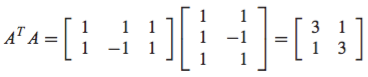
\includegraphics[width=6cm]{figs/4-1-1_Normal_Equations-1} 
%\caption{$f(x) = x^3 + x -1$的图像} 
\end{figure}
以及
\begin{figure}
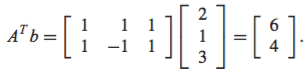
\includegraphics[width=5cm]{figs/4-1-1_Normal_Equations-2} 
%\caption{$f(x) = x^3 + x -1$的图像} 
\end{figure}
\end{frame}


\begin{frame}
\frametitle{最小二乘解举例}
从而我们得到法方程组
\begin{align}
&\left[ \begin{array}{cc}
     3    & 1 \\
     1    &   3 \\                         
            \end{array} \right] 
\left[ \begin{array}{c} 
      x_1 \\ x_2 \end{array} \right] 
=
\left[ \begin{array}{c}
      6 \\4  \end{array} \right].
\end{align}
解得$\bar{x} = (\frac{7}{4}, \frac{3}{4})$。将解代入原方程得
\begin{figure}
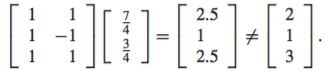
\includegraphics[width=6cm]{figs/4-1-1_Example-1-1} 
%\caption{$f(x) = x^3 + x -1$的图像} 
\end{figure}
而
\begin{figure}
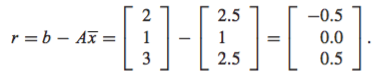
\includegraphics[width=6cm]{figs/4-1-1_Example-1-2} 
%\caption{$f(x) = x^3 + x -1$的图像} 
\end{figure}
\end{frame}


\begin{frame}
\frametitle{残量的三种解释}
考虑残量$r = Ax - b$,我们可以利用残量给出三种不同的误差度量。

\vspace{0.2cm}

首先是误差的2-范数,或者残量的欧几里得长度,即
\begin{equation}
\|r\|_2 = \sqrt{r_1^2 + \ldots +r_m^2}.
\end{equation}

第二个是平方误差(sqaured error),即
\begin{equation}
SE = r_1^2 + \ldots + r_m^2.
\end{equation}

第三个是均方差根(root mean squared error),即
\begin{equation}
RMSE = \sqrt{\frac{SE}{m}} = \sqrt{\frac{r_1^2 + \ldots + r_m^2}{m}} = \frac{\sqrt{SE}}{\sqrt{m}} = \frac{\|r\|_2}{\sqrt{m}}.
\end{equation}
\end{frame}


%%%%%%%%%%%%%%%%%%%%%%%%%%%%%%%%%%%%%%%%%%

\section{最小二乘数据拟合}

\begin{frame}
\frametitle{数据拟合}
考虑数据点$(t_1,y_1), (t_2, y_2), \ldots, (t_m, y_m)$。如果给定一个类型的模型,例如直线$y = c_1 + c_2 t$,我们提出这样一个问题:如何确定参数$c_1, c_2$的值使得这条直线在$2-$范数意义下对这些数据点作了最好的拟合。

\vspace{0.2cm}

如果将上面的语言变为数学语言,那么这等价于:找到参数$c_1, c_2$,使得数据点关于直线$y = c_1 + c_2 t$的残量的平方和最小。可以见下图
\begin{figure}
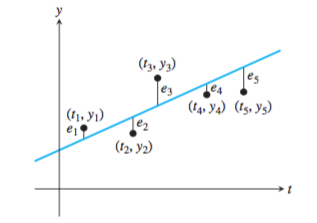
\includegraphics[width=6cm]{figs/4-1-2_Fitting_Data-1} 
%\caption{$f(x) = x^3 + x -1$的图像} 
\end{figure}
\end{frame}


\begin{frame}
\frametitle{数据拟合}
我们注意到两点:
\begin{enumerate}
\item 首先,数据拟合与插值有相似之处,都是利用数据点寻找生成数据点的函数的某个近似函数。但是插值的条件一般是近似函数要过给定的数据点,但近似函数的形式是可变的;而拟合不要求近似函数过每一个数据点,但近似函数的形式是不变的。
\item 其次,我们发现经过数据点$(t_i, y_i)$作垂直于$t-$轴(或平行于$y-$轴)的直线,这条直线与直线$y = c_1 + c_2t$的交点与$(t_i, y_i)$的距离刚好是$|e_i| = |y_i - (c_1 + c_2 t_i)|$,其中$e_i$是数据点$(t_i, y_i)$关于直线$y = c_1 + c_2 t$的残量。
\end{enumerate}

我们可以通过以下的例子来寻找数据拟合和最小二乘之间的关系。
\end{frame}


\begin{frame}
\frametitle{数据拟合与最小二乘}
\begin{example}
寻找数据点$(x_1, y_1) = (1,2), (t_2, y_2) = (-1,1), (t_3, y_3) = (1,3)$在残量平方最小意义下的最佳拟合直线。
\end{example}
我们设这条直线的方程为
\begin{equation}
y = c_1 + c_2 t.
\end{equation}
如果存在一条直线通过这三个点,那么这条直线一定满足以下方程组
\begin{align}
c_1 + c_2 t_1 = c_1 + c_2 (1) = 2 &= y_1, \nonumber \\
c_1 + c_2 t_2 = c_1 + c_2 (-1) = 1 &= y_2, \nonumber \\
c_1 + c_2 t_3 = c_1 + c_2 (1) = 3 &= y_3.
\end{align}
\end{frame}


\begin{frame}
\frametitle{数据拟合与最小二乘}
化为矩阵形式$Ac = b$就是
\begin{align}
Ac = &\left[ \begin{array}{cc}
     1    & 1 \\
     1    &   -1 \\
     1    & 1                         
            \end{array} \right] 
\left[ \begin{array}{c} 
      c_1 \\ c_2 \end{array} \right] 
=
\left[ \begin{array}{c}
      2 \\ 1 \\ 3  \end{array} \right] = b.
\end{align}
但是事实上,上面的方程组是没有解的,这是因为从几何上说,上面这三个数据点不在一条直线上,而从代数上说,上面的方程组中第一个方程和第三个方程无法同时满足。这时我们发现,由于我们寻找的是残量平方意义下的最佳拟合直线,而根据之前对数据点关于直线的残量的定义,我们发现由三个数据点关于直线的残量$e_1, e_2, e_3$构成的向量$r$恰好满足$r = b - Ac$。

\vspace{0.2cm}

这样,要求残量平方意义下的最佳拟合直线就等价于可以对上面的方程组$Ac = b$求最小二乘意义下的解。最后得到$(c_1, c_2) = (\frac{7}{4}, \frac{3}{4})$,进而我们所求直线为$y = \frac{7}{4} + \frac{3}{4}t$。
\end{frame}


\begin{frame}
\frametitle{数据拟合与最小二乘}
将数据点回代入直线方程组,可以得到下表
\begin{figure}
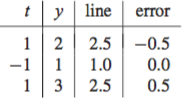
\includegraphics[width=3cm]{figs/4-1-2_Fitting_Data-2} 
%\caption{$f(x) = x^3 + x -1$的图像} 
\end{figure}
可以计算得这个计算结果的均方差根为$\frac{1}{\sqrt{6}}$。解的几何表示如下图
\begin{figure}
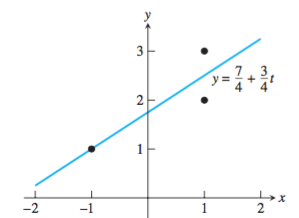
\includegraphics[width=5cm]{figs/4-1-2_Fitting_Data-3} 
%\caption{$f(x) = x^3 + x -1$的图像} 
\end{figure}
\end{frame}


\begin{frame}
\frametitle{最小二乘拟合}
通过上面的方法得到数据拟合称为最小二乘拟合。给定$m$个数据点$(t_1, y_1), \ldots, (t_m, y_m)$,最小二乘拟合一般分为三个步骤:

\begin{enumerate}
\item 选择模型:选择一个带参数的模型,例如我们之前选取的线性模型$ y = c_1 + c_2t$。
\item “迫使”模型满足数据:将数据点代入模型,一个数据点会生成一个关于模型参数(例如$c_1$和$c_2$)的线性方程,进而得到一个线性方程组$Ax = b$,其中$x$表示的是未知的模型参数。
\item 解法方程:解关于参数的线性方程组的法方程$A^TAx = A^Tb$,得到模型的参数。
\end{enumerate}
\end{frame}


\begin{frame}
\frametitle{最小二乘拟合举例}
\begin{example}
对数据点$(-1,1), (0,0), (1,0), (2, -2)$利用直线和双曲线进行最小二乘拟合。
\end{example}
首先设拟合曲线为$y = c_1 + c_2 t$。代入数据点得到方程组
\begin{align}
c_1 + c_2 (-1) = 1 \nonumber \\
c_1 + c_2 (0) = 0 \nonumber \\
c_1 + c_2 (1) = 0 \nonumber \\
c_1 + c_2 (2) = -2.
\end{align}
写成矩阵形式就是
\begin{align}
&\left[ \begin{array}{cc}
     1    & -1 \\
     1    &   0 \\
     1    & 1  \\
     1    & 2                       
            \end{array} \right] 
\left[ \begin{array}{c} 
      c_1 \\ c_2 \end{array} \right] 
=
\left[ \begin{array}{c}
      1 \\ 0 \\ 0  \\ -2  \end{array} \right] .
\end{align}
\end{frame}


\begin{frame}
\frametitle{最小二乘拟合举例}
计算得上面的方程组的法方程组为
\begin{align}
\left[ \begin{array}{cc}
     4    & 2 \\
     2    &   6                 
            \end{array} \right] 
\left[ \begin{array}{c} 
      c_1 \\ c_2 \end{array} \right] 
=
\left[ \begin{array}{c}
      -1 \\ -5   \end{array} \right] .
\end{align}
解得最佳拟合直线方程为$y = c_1 + c_2t = 0.2 - 0.9t$。
将数据点回代入直线方程组,可以得到下表
\begin{figure}
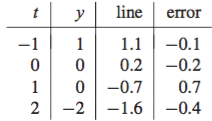
\includegraphics[width=3.5cm]{figs/4-1-2_Fitting_Data-4} 
%\caption{$f(x) = x^3 + x -1$的图像} 
\end{figure}
计算得$SE = 0.7$而$RMSE = \sqrt{\frac{0.7}{4}} \approx 0.418$.
\end{frame}


\begin{frame}
\frametitle{最小二乘拟合举例}
我们现在将拟合模型变为双曲线模型,即令
\begin{equation}
y = c_1 + c_2 t + c_3 t^2.
\end{equation}
代入数据得到方程组
\begin{align}
c_1 + c_2 (-1) + c_3 (-1)^2 = 1 \nonumber \\
c_1 + c_2 (0) + c_3(0)^2 = 0 \nonumber \\
c_1 + c_2 (1) + c_3 (1)^2 = 0 \nonumber \\
c_1 + c_2 (2) + c_3 (2)^2 = -2.
\end{align}
\end{frame}


\begin{frame}
\frametitle{最小二乘拟合举例}
以上方程写为矩阵形式得到
\begin{align}
&\left[ \begin{array}{ccc}
     1    & -1 & 1\\
     1    &   0 & 0\\
     1    & 1  & 1\\
     1    & 2  & 4                     
            \end{array} \right] 
\left[ \begin{array}{c} 
      c_1 \\ c_2 \\ c_3 \end{array} \right] 
=
\left[ \begin{array}{c}
      1 \\ 0 \\ 0  \\ -2  \end{array} \right] .
\end{align}
则方程组的法方程为
\begin{align}
&\left[ \begin{array}{ccc}
     4    & 2 & 6\\
     2    &   6 & 8\\
     6    & 8  & 18\\                   
            \end{array} \right] 
\left[ \begin{array}{c} 
      c_1 \\ c_2 \\ c_3 \end{array} \right] 
=
\left[ \begin{array}{c}
      -1 \\ -5 \\ -7   \end{array} \right] .
\end{align}
解得拟合曲线
\begin{equation}
y = c_1 + c_2 t + c_3 t^2 = 0.45 - 0.65t -0.25t^2.
\end{equation} 
\end{frame}


\begin{frame}
\frametitle{最小二乘拟合举例}
将数据点回代入直线方程组,可以得到下表
\begin{figure}
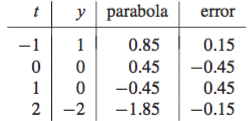
\includegraphics[width=4cm]{figs/4-1-2_Fitting_Data-5} 
%\caption{$f(x) = x^3 + x -1$的图像} 
\end{figure}
计算得$SE = 0.45$而$RMSE = \sqrt{\frac{0.45}{4}} \approx 0.335$.

\vspace{0.2cm}

这个例子告诉我们,我们不仅可以利用直线进行数据拟合,只要模型曲线的参数是以线性的方式呈现出来的,我们都可以利用最小二乘拟合计算数据的最佳拟合曲线。
\end{frame}


%%%%%%%%%%%%%%%%%%%%%%%%%%%%%%%%%%%%%%%%%%



\section{数据拟合模型}


\begin{frame}
\frametitle{数据拟合模型}
之前我们考虑了利用多项式模型对数据进行拟合。实际上,我们还有很多其它的数据拟合模型可以选择,这些模型有些是根据数据产生的物理原理得到的,有些是根据经验得到的。
\end{frame}


\subsection{周期性数据}

\begin{frame}
\frametitle{周期性数据}
周期性数据往往是由周期性的现象产生的,例如气温就是一个很好的具有周期性的数据,每天、每年都可以作为周期。我们最为熟知的周期性函数就是正弦和余弦函数,因此我们的模型就是基于正余弦函数得到的。

\begin{example}
利用周期性模型对根据以下某天的气温情况进行数据拟合。
\begin{figure}
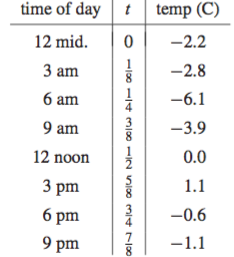
\includegraphics[width=3.8cm]{figs/4-2-1_Perriodic_Data-1} 
%\caption{$f(x) = x^3 + x -1$的图像} 
\end{figure}
\end{example}
\end{frame}


\begin{frame}
\frametitle{周期性数据}
我们首先选取$y = c_1 + c_2 \cos 2\pi t + c_3 \sin 2\pi t$作为我们的模型。代入数据得到方程组
\begin{figure}
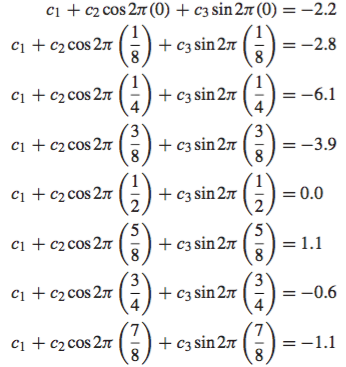
\includegraphics[width=5cm]{figs/4-2-1_Perriodic_Data-2} 
%\caption{$f(x) = x^3 + x -1$的图像} 
\end{figure}
\end{frame}


\begin{frame}
\frametitle{周期性数据}
将方程组写为$Ax = b$的形式,我们得到
\begin{figure}
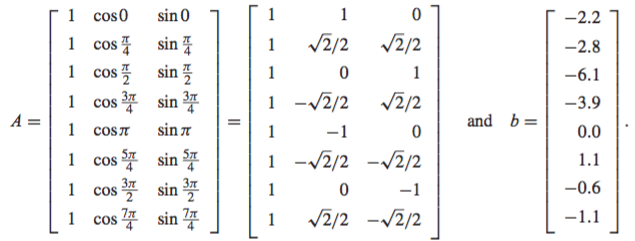
\includegraphics[width=10cm]{figs/4-2-1_Perriodic_Data-3} 
%\caption{$f(x) = x^3 + x -1$的图像} 
\end{figure}
\end{frame}


\begin{frame}
\frametitle{周期性数据}
通过计算,我们得到法方程组$A^TA c = A^Tb$为
\begin{align}
&\left[ \begin{array}{ccc}
     8    & 0   & 0\\
     0    &   4 & 0\\
     0    & 0  & 4\\                   
            \end{array} \right] 
\left[ \begin{array}{c} 
      c_1 \\ c_2 \\ c_3 \end{array} \right] 
=
\left[ \begin{array}{c}
      -15.6 \\ -2.9778 \\ -10.2376   \end{array} \right] .
\end{align}
解得$c_1 = -1.95, c_2 = -0.7445, c_3 = -2.5594$。进而得到最佳逼近模型
\begin{equation}
y = -1.95 - 0.7445 \cos 2 \pi t - 2.5594 \sin 2\pi t.
\end{equation}
而$RMSE \approx 1.063$。
\end{frame}


\begin{frame}
\frametitle{周期性数据}
我们再选取$y = c_1 + c_2 \cos 2\pi t + c_3 \sin 2\pi t + c_4 \cos 4 \pi t$作为我们的模型。代入数据得到方程组
\begin{figure}
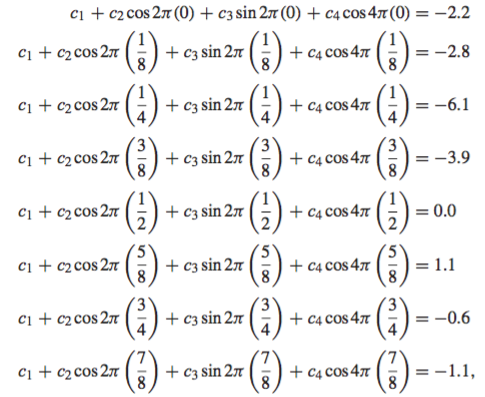
\includegraphics[width=8cm]{figs/4-2-1_Perriodic_Data-4} 
%\caption{$f(x) = x^3 + x -1$的图像} 
\end{figure}
\end{frame}


\begin{frame}
\frametitle{周期性数据}
通过计算,我们得到法方程组为
\begin{align}
&\left[ \begin{array}{cccc}
     8    & 0   & 0  & 0 \\
     0    &   4 & 0 & 0\\
     0    & 0  & 4  & 0 \\
     0    &  0 & 0  &4                   
            \end{array} \right] 
\left[ \begin{array}{c} 
      c_1 \\ c_2 \\ c_3 \\c_4 \end{array} \right] 
=
\left[ \begin{array}{c}
      -15.6 \\ -2.9778 \\ -10.2376 \\ 4.5  \end{array} \right] .
\end{align}
解得$c_1 = -1.95, c_2 = -0.7445, c_3 = -2.5594, c_4 = 1.125$。进而得到最佳逼近模型
\begin{equation}
y = -1.95 - 0.7445 \cos 2 \pi t - 2.5594 \sin 2\pi t + 1.125 \cos 4 \pi t.
\end{equation}
而$RMSE \approx 0.705$。
\end{frame}


\begin{frame}
\frametitle{周期性数据}
两个模型对数据的拟合情况如下图所示
\begin{figure}
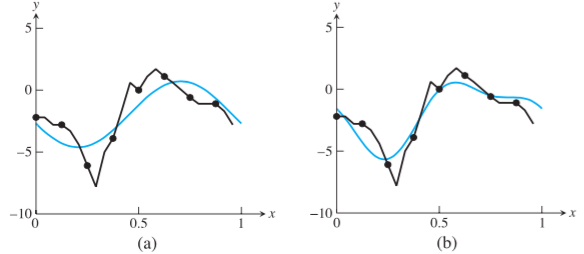
\includegraphics[width=10cm]{figs/4-2-1_Perriodic_Data-5} 
%\caption{$f(x) = x^3 + x -1$的图像} 
\end{figure}
很明显第二个模型的拟合效果比第一个模型的拟合效果好。
\end{frame}


\begin{frame}
\frametitle{正交性}
我们发现一个有趣的现象:上面两个模型导出的法方程组的系数矩阵都是对角矩阵。这意味着解系数$c_1, c_2, c_3$变得非常简单。

\vspace{0.2cm}

这个现象不是偶然的,事实上,通过基函数(即这里的$\sin$、$\cos$函数)的特殊选取,我们可以将法方程组变得相对简单。这个问题我们将在下一讲当中涉及。
\end{frame}


\subsection{数据线性化}

\begin{frame}
\frametitle{指数增长模型}
在环境条件允许的情况下,物种的增长大体符合指数增长模型,即
\begin{equation}
\label{eq: exponential growth}
y = c_1 e^{c_2 t},
\end{equation}
其中$y$是种群数量,$t$是时间。如果我们有对种群数量的在某些时刻的计量或者估计值,如何通过这些数据估计参数$c_1$和$c_2$呢?

\vspace{0.2cm}

很明显,由于$c_1$和$c_2$已经不是线性关系了,所以不能够直接代入数据利用法方程组来进行求解。这里我们有两种途径对参数求解:
\begin{enumerate}
\item 将数据直接代入,将残量最小化,也就是最小化$\sum_{i = 1}^{m} |y_i - c_1 e^{c_2 t_i}|^2$这个值,以求得$c_1$和$c_2$。这种方法称为非线性最小二乘方法。
\item 将数据进行处理,使得参数满足线性的关系,这就是数据线性化方法。
\end{enumerate}

我们这里着重讨论数据线性化方法。
\end{frame}


\begin{frame}
\frametitle{指数增长模型}
对于指数增长模型\eqref{eq: exponential growth},我们两边同时取$\ln$得到
\begin{equation}
\ln y = \ln(c_1 e^{c_2 t}) = \ln c_1 + c_2 t.
\end{equation}
之后令$k = \ln c_1$,则
\begin{equation}
\ln y = k + c_2 t.
\end{equation}
这样$k$和$c_2$就是一个线性的关系了。代入数据就可以得到关于$k$和$c_2$的超定方程组,利用法方程组可以解得最小二乘意义下的$k$和$c_1$的值。

\vspace{0.2cm}

需要注意的是,利用数据线性化求得的最小二乘意义的解实际上是最小化了
\begin{equation}
\sum_{i = 1}^{m}(\ln c_i + c_2 t_i - \ln y_i)^2.
\end{equation}

直接的非线性最小二乘法和线性化之后的最小二乘法并没有优劣之分,这两种方法的适用性需要对数据拟合的问题进行分析才能得出结论。
\end{frame}


\begin{frame}
\frametitle{指数增长模型举例}
\begin{example}
利用指数增长模型$y = c_1 e^{c_2 t}$对世界上的轿车数量进行数据拟合
\begin{figure}
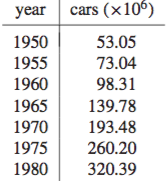
\includegraphics[width=3cm]{figs/4-2-2_Exponential_Growth-1} 
%\caption{$f(x) = x^3 + x -1$的图像} 
\end{figure}
\end{example}
利用数据线性化的技巧可以得到$k \approx 3.9896$,$c_2 \approx 0.06152$。因此$c_1 \approx e^{3.9896} \approx 54.03$,所以模型为
\begin{equation}
y = 54.03 e^{0.06152t}.
\end{equation}
\end{frame}


\begin{frame}
\frametitle{指数增长模型举例}
如果代入数据和模型进一步计算,我们可以得到线性化后的模型的$RMSE$大约是0.0357,而原模型的残量$r$的$2-$范数是9.56。模型与数据的关系如下图
\begin{figure}
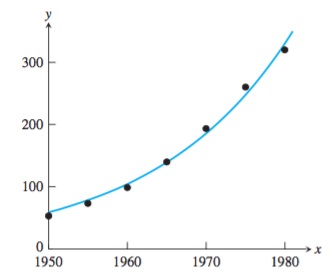
\includegraphics[width=6cm]{figs/4-2-2_Exponential_Growth-2} 
%\caption{$f(x) = x^3 + x -1$的图像} 
\end{figure}
\end{frame}


\begin{frame}
\frametitle{指数增长模型举例}
\begin{example}
利用指数增长模型$y = c_1 e^{c_2 t}$对Intel处理器中的晶体管的数量进行数据拟合
\begin{figure}
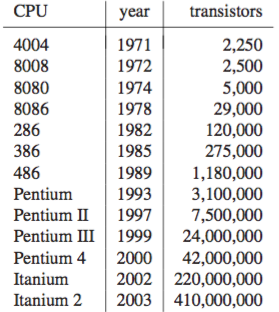
\includegraphics[width=4cm]{figs/4-2-2_Exponential_Growth-3} 
%\caption{$f(x) = x^3 + x -1$的图像} 
\end{figure}
\end{example}
\end{frame}


\begin{frame}
\frametitle{指数增长模型举例}
仍然设模型为
\begin{equation}
y = c_1 e^{c_2 t}.
\end{equation}
这时候如果将$t$代为表上的数据显然是没有意义的,因为晶体管诞生的时间很晚,根本不需要考虑1950年以前的情况。因此,我们将$1970$年设为$t = 0$,将年代的信息重新计算得到
\begin{align}
k + c_2 * 1= \ln 2250 \nonumber \\
k + c_2 * 2= \ln 2500 \nonumber \\
k + c_2 * 4= \ln 5000 \nonumber \\
k + c_2 * 8= \ln 29000,
\end{align}
等等。其中$k = \ln c_1$。通过计算,我们最终可以得到法方程组
\begin{align}
&\left[ \begin{array}{cc}
     13    & 235    \\
     235    &   5927         
            \end{array} \right] 
\left[ \begin{array}{c} 
      k \\ c_2  \end{array} \right] 
=
\left[ \begin{array}{c}
      176.9 \\ 3793.23  \end{array} \right] .
\end{align}
\end{frame}


\begin{frame}
\frametitle{指数增长模型举例}
计算得$k \approx 7.197$,$c_2 \approx 0.3546$,因此$c_1  \approx 1335.3$,进而
\begin{equation}
y = 1335.3 e^{0.3546 t}.
\end{equation}
拟合的效果如下图所示
\begin{figure}
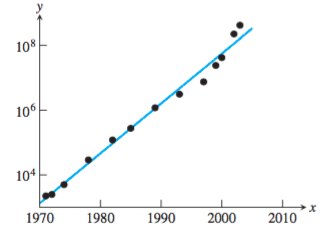
\includegraphics[width=4.5cm]{figs/4-2-2_Exponential_Growth-4} 
%\caption{$f(x) = x^3 + x -1$的图像} 
\end{figure}
晶体管的数量翻倍的时间大约为$\frac{\ln 2}{c_2} \approx 1.95$年。这就是著名的Moore定理。我们在上图也注意到,晶体管数量的在2000年以后有了一个明显的加速增加。
\end{frame}


\begin{frame}
\frametitle{幂法则模型}
除了指数增长模型外,另一个重要的模型是幂法则模型,也就是说
\begin{equation}
y = c_1 t^{c_2}.
\end{equation}
我们将两边同时取$\ln$,得到
\begin{equation}
\ln y = \ln c_1 + c_2 \ln t = k + c_2 \ln t.
\end{equation}
代入数据得到超定方程的系数矩阵和右端项分别为
\begin{figure}
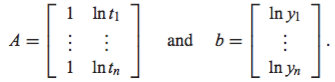
\includegraphics[width=6cm]{figs/4-2-2_Power_Law-1} 
%\caption{$f(x) = x^3 + x -1$的图像} 
\end{figure}
\end{frame}


\begin{frame}
\frametitle{幂法则模型举例}
\begin{example}
利用幂法则模型对以下儿童身高体重模型数据进行拟合
\begin{figure}
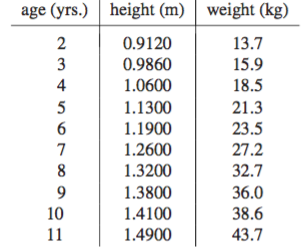
\includegraphics[width=6cm]{figs/4-2-2_Power_Law-2} 
%\caption{$f(x) = x^3 + x -1$的图像} 
\end{figure}
\end{example}
\end{frame}


\begin{frame}
\frametitle{幂法则模型举例}
利用之前的幂法则,设体重是身高的函数,得到
\begin{equation}
W = 16.3 H^{2.42}.
\end{equation}
拟合结果如下图
\begin{figure}
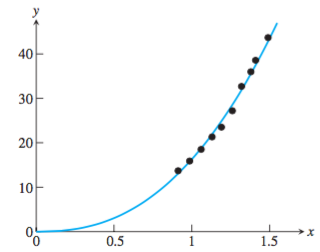
\includegraphics[width=5cm]{figs/4-2-2_Power_Law-3} 
%\caption{$f(x) = x^3 + x -1$的图像} 
\end{figure}
有趣的是,我们可以把以上拟合结果中的16.3看作是人体的平均密度,而2.42是人体关于身高的“平均维度”。
\end{frame}


\begin{frame}
\frametitle{药代动力学模型}
一般来说,药物在血液中的浓度与时间的关系近似的满足
\begin{equation}
y = c_1 t e^{c_2 t},
\end{equation}
其中$t$是吃药后的时间。这个模型的特点是浓度$y$随着时间快速上升,之后进入一个缓慢的指数衰减期。药物的半衰期是只药物从浓度最高的时刻到浓度减为一半时刻之间的时间长度。

\vspace{0.2cm}

对于这个模型,我们两边同时取$\ln$,得到
\begin{align}
\ln y &= \ln c_1 + \ln t + c_2 t \nonumber \\
k + c_2 t &= \ln y - \ln t,
\end{align}
其中$k = \ln c_1$。
\end{frame}


\begin{frame}
\frametitle{药代动力学模型}
代入数据得到超定方程组$Ax = b$,其中
\begin{figure}
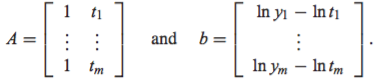
\includegraphics[width=8cm]{figs/4-2-2_Drug_Concentration-1} 
%\caption{$f(x) = x^3 + x -1$的图像} 
\end{figure}
解该方程组的法方程得到$k$和$c_2$,其中$c_1 = e^k$。
\end{frame}


\begin{frame}
\frametitle{药代动力学模型举例}
\begin{example}
一个病人在吃药后血液中药物浓度如下表,
\begin{figure}
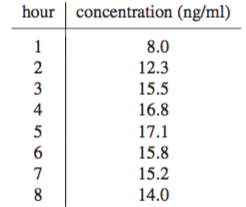
\includegraphics[width=4cm]{figs/4-2-2_Drug_Concentration-2} 
%\caption{$f(x) = x^3 + x -1$的图像} 
\end{figure}
求药代动力学模型的参数。
\end{example}
\end{frame}


\begin{frame}
\frametitle{药代动力学模型举例}
根据药代动力学模型,代入解得
\begin{equation}
y = 9.77 t e^{-0.215t}.
\end{equation}
拟合结果如下图
\begin{figure}
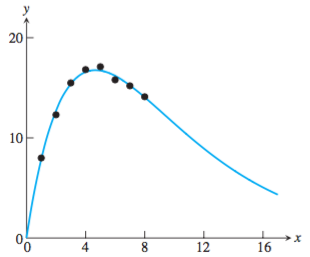
\includegraphics[width=5cm]{figs/4-2-2_Drug_Concentration-3} 
%\caption{$f(x) = x^3 + x -1$的图像} 
\end{figure}
\end{frame}

%%%%%%%%%%%%%%%%%%%%%%%%%%%%%%%%%%%%%%%%%%

\begin{frame}
\frametitle{课后阅读及作业}
[NA] 第4章 4.1.1,4.1.2,4.2 \\
作业:[NA] 4.1:2,3,6,8,9,11;4.2: 1,3,5,6。


\end{frame}

\end{document}

